\chapter{Architettura hardware}
%\markboth{Introduzione}{Introduzione}
\label{cap:architettura}

In questo capitolo viene descritta in dettaglio la componentistica hardware utilizzata per l'implementazione del gioco.

\section{Unità di elaborazione}
L'elaborazione dei dati trasmessi dal robot e la definizione dei comportamenti in base alle logiche di gioco sono gestiti da un elaboratore esterno, che viene anche utilizzato dal giocatore per controllare lo stato del gioco (punteggio, tempo rimanente, \dots) e gestirne l'avvio.

\section{Il robot}

L'attore principale del gioco è il robot autonomo \emph{Spykee}, un modello commerciale della Meccano \cite{spykeeweb}, disponibile nel laboratorio di Intelligenza Artificiale e Robotica (AIRLab) del Politecnico di Milano. Questo modello è già stato utilizzato con successo in precedenti progetti nell'ambito dei Robogame\footnote{in particolare nelle varie versioni di Robowii \cite{robowii} }.

Spykee si muove tramite due cingoli (con tecnica differential drive). Una telecamera montata sulla testa permette di catturare immagini fortemente compresse in formato JPEG con una risoluzione di $320 \times 240$ pixel a una frequenza di circa $20$ frame al secondo. Per comunicare con il computer che effettua il controllo, viene utilizzata una rete Wi-Fi. Delle varie modalità di connessione messe a disposizione dal robot, viene utilizzata la modalità ``local ad hoc mode'': il robot crea all'accensione una rete Wi-Fi ad-hoc a cui il computer deve essere connesso.

\begin{figure}[h]
\centering
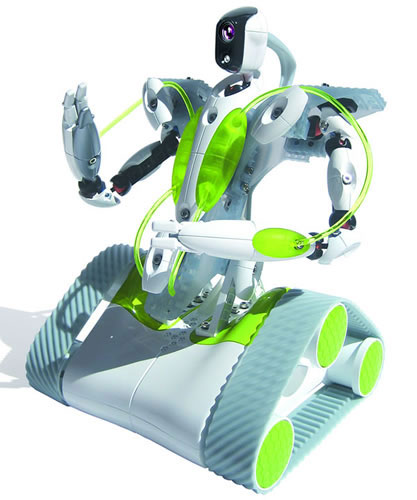
\includegraphics[scale=0.2]{images/spykee}
\caption{Il robot Spykee}
\end{figure}

\subsection*{Aggiunte hardware}
A partire da quanto già realizzato nei precedenti progetti, Spykee è stato dotato di ulteriori sensori che lo rendono adatto all'utilizzo all'interno del gioco. Tutti i componenti hardware aggiunti al robot sono controllati da un microcontrollore. A questo scopo è stata utilizzata una scheda STM32F4 Discovery Board della ST \cite{st}, dotata di un processore ARM Cortex M4, scelta per le sue caratteristiche: in particolare il grande numero di periferiche (GPIO, timer, interfacce seriali) utilizzabili.

Il firmware realizzato per controllare i vari dispositivi è stato sviluppato utilizzando il sistema operativo ChibiOS/RT \cite{chibios}. L'utilizzo di un sistema operativo per microcontrollori permette sia di utilizzare concetti di programmazione concorrente quali thread e mutex, che di astrarre l'hardware sottostante, consentendo quindi una certa modularità (ottenuta isolando ogni funzione in un thread indipendente) e quindi un rapido sviluppo del firmware.

La scheda comunica con l'unità di elaborazione tramite un collegamento wireless di tipo Zigbee (utilizzando un modulo XBee della Digi). Il protocollo è caratterizzato da una bassa velocità di trasmissione (comunque ampiamente sufficiente per gli scopi del progetto), ma da una buona facilità di utilizzo, specialmente in ambito embedded: nella modalità più semplice viene infatti utilizzato come un collegamento seriale punto-punto tra microcontrollore e computer.

Tutti i vari componenti sono state raccolti in una apposita scatola e sono alimentati direttamente dal pacco batteria di Spykee tramite un regolatore di tensione, che permette di ridurre la tensione proveniente dalla batteria (circa $9$ V) a quella di $5$ V. Un apposito interruttore, posto a valle dell'interruttore di alimentazione di Spykee, permette di spegnere o accendere le aggiunte hardware\footnote{Durante la carica delle batterie, si consiglia di tenere spente le aggiunte hardware}.

\paragraph{Sonar} Per rilevare, e quindi evitare, eventuali ostacoli incontrati durante il movimento del robot, sono stati montati quattro sonar MaxSonar\textregistered-EZ della MaxBotix, uno per ognuno dei punti cardinali (nord, sud, ovest, est). L'aggiunta di un certo numero di sensori è necessaria in quanto il robot non è progettato per muoversi autonomamente, ma soltanto per ricevere comandi impartiti manualmente. 

\paragraph{Led} Spykee è stato dotato di due strisce di LED (quattro LED gialli e quattro rossi) e di un LED verde che permettono di mostrare alcune informazioni relative allo stato del robot e/o del gioco nel complesso. Sul robot sono anche presenti due led a infrarossi, che venivano utilizzati insieme a un controller Wiimote in precedenti progetti, ma che non sono di interesse per questo gioco. 

\begin{figure}
\centering
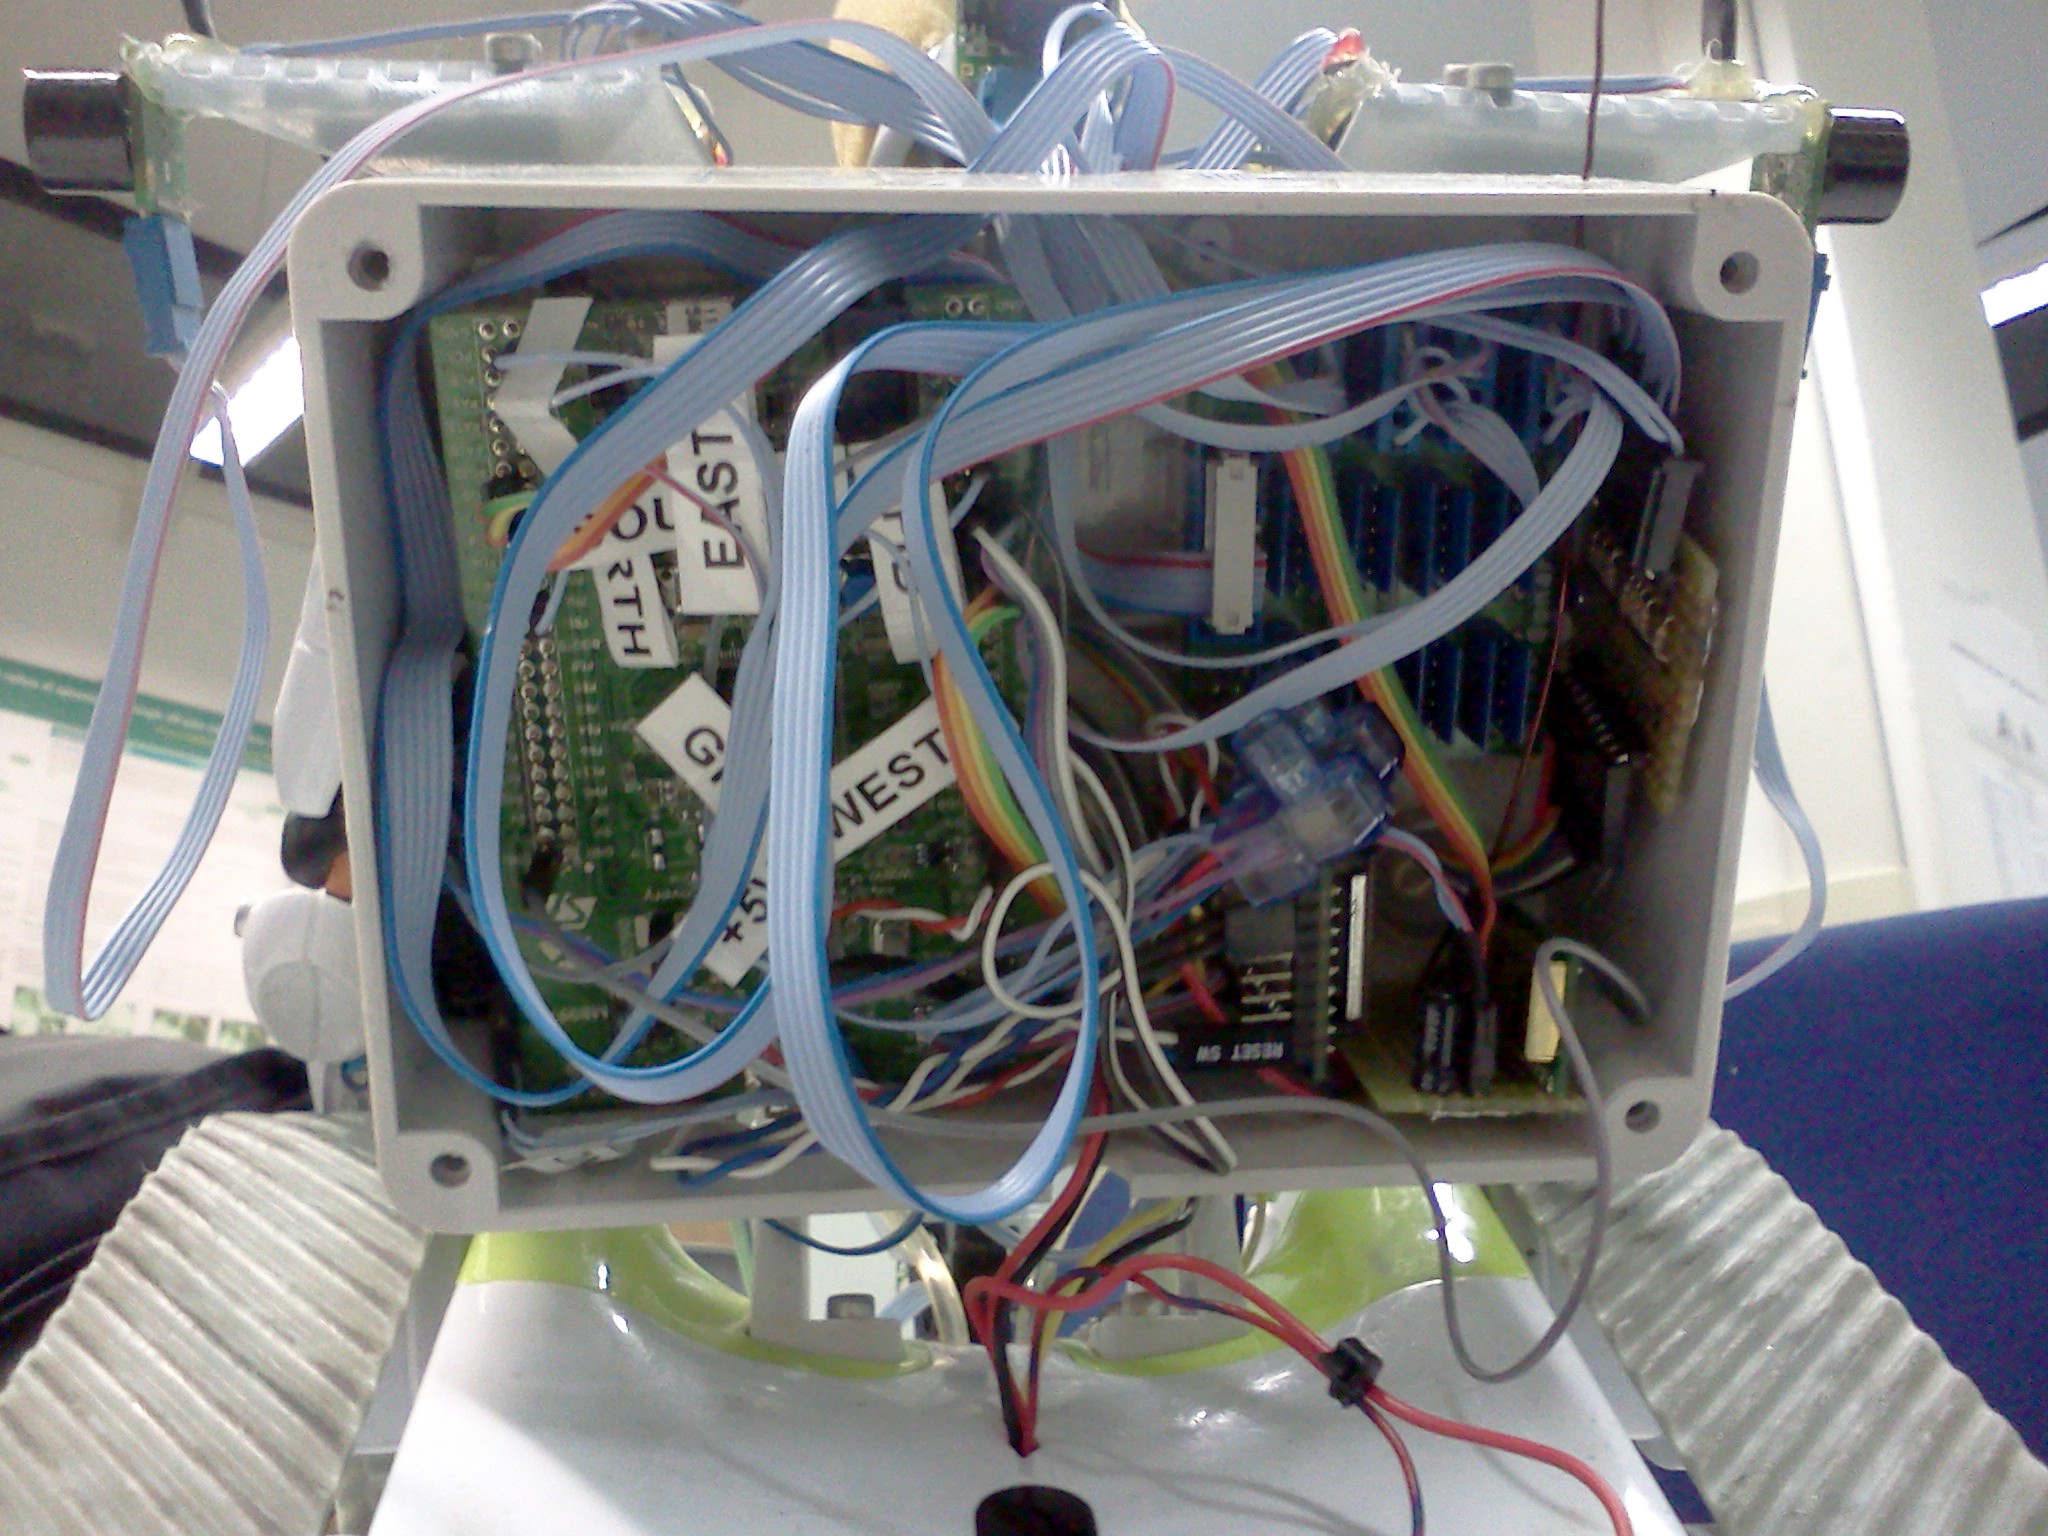
\includegraphics[scale=0.14]{images/scatola}
\caption{La scatola con i componenti che sono stati aggiunti al robot}
\end{figure}

\noindent Le altre aggiunte hardware sono strettamente collegate ad altri componenti del gioco, pertanto verranno descritte nei paragrafi successivi.


\section{Ostacoli attivi}
Per quanto riguarda l'implementazione delle \emph{trappole} (gli ostacoli che modificano il comportamento del robot) sono state valutate diverse soluzioni.

\begin{figure}
\centering
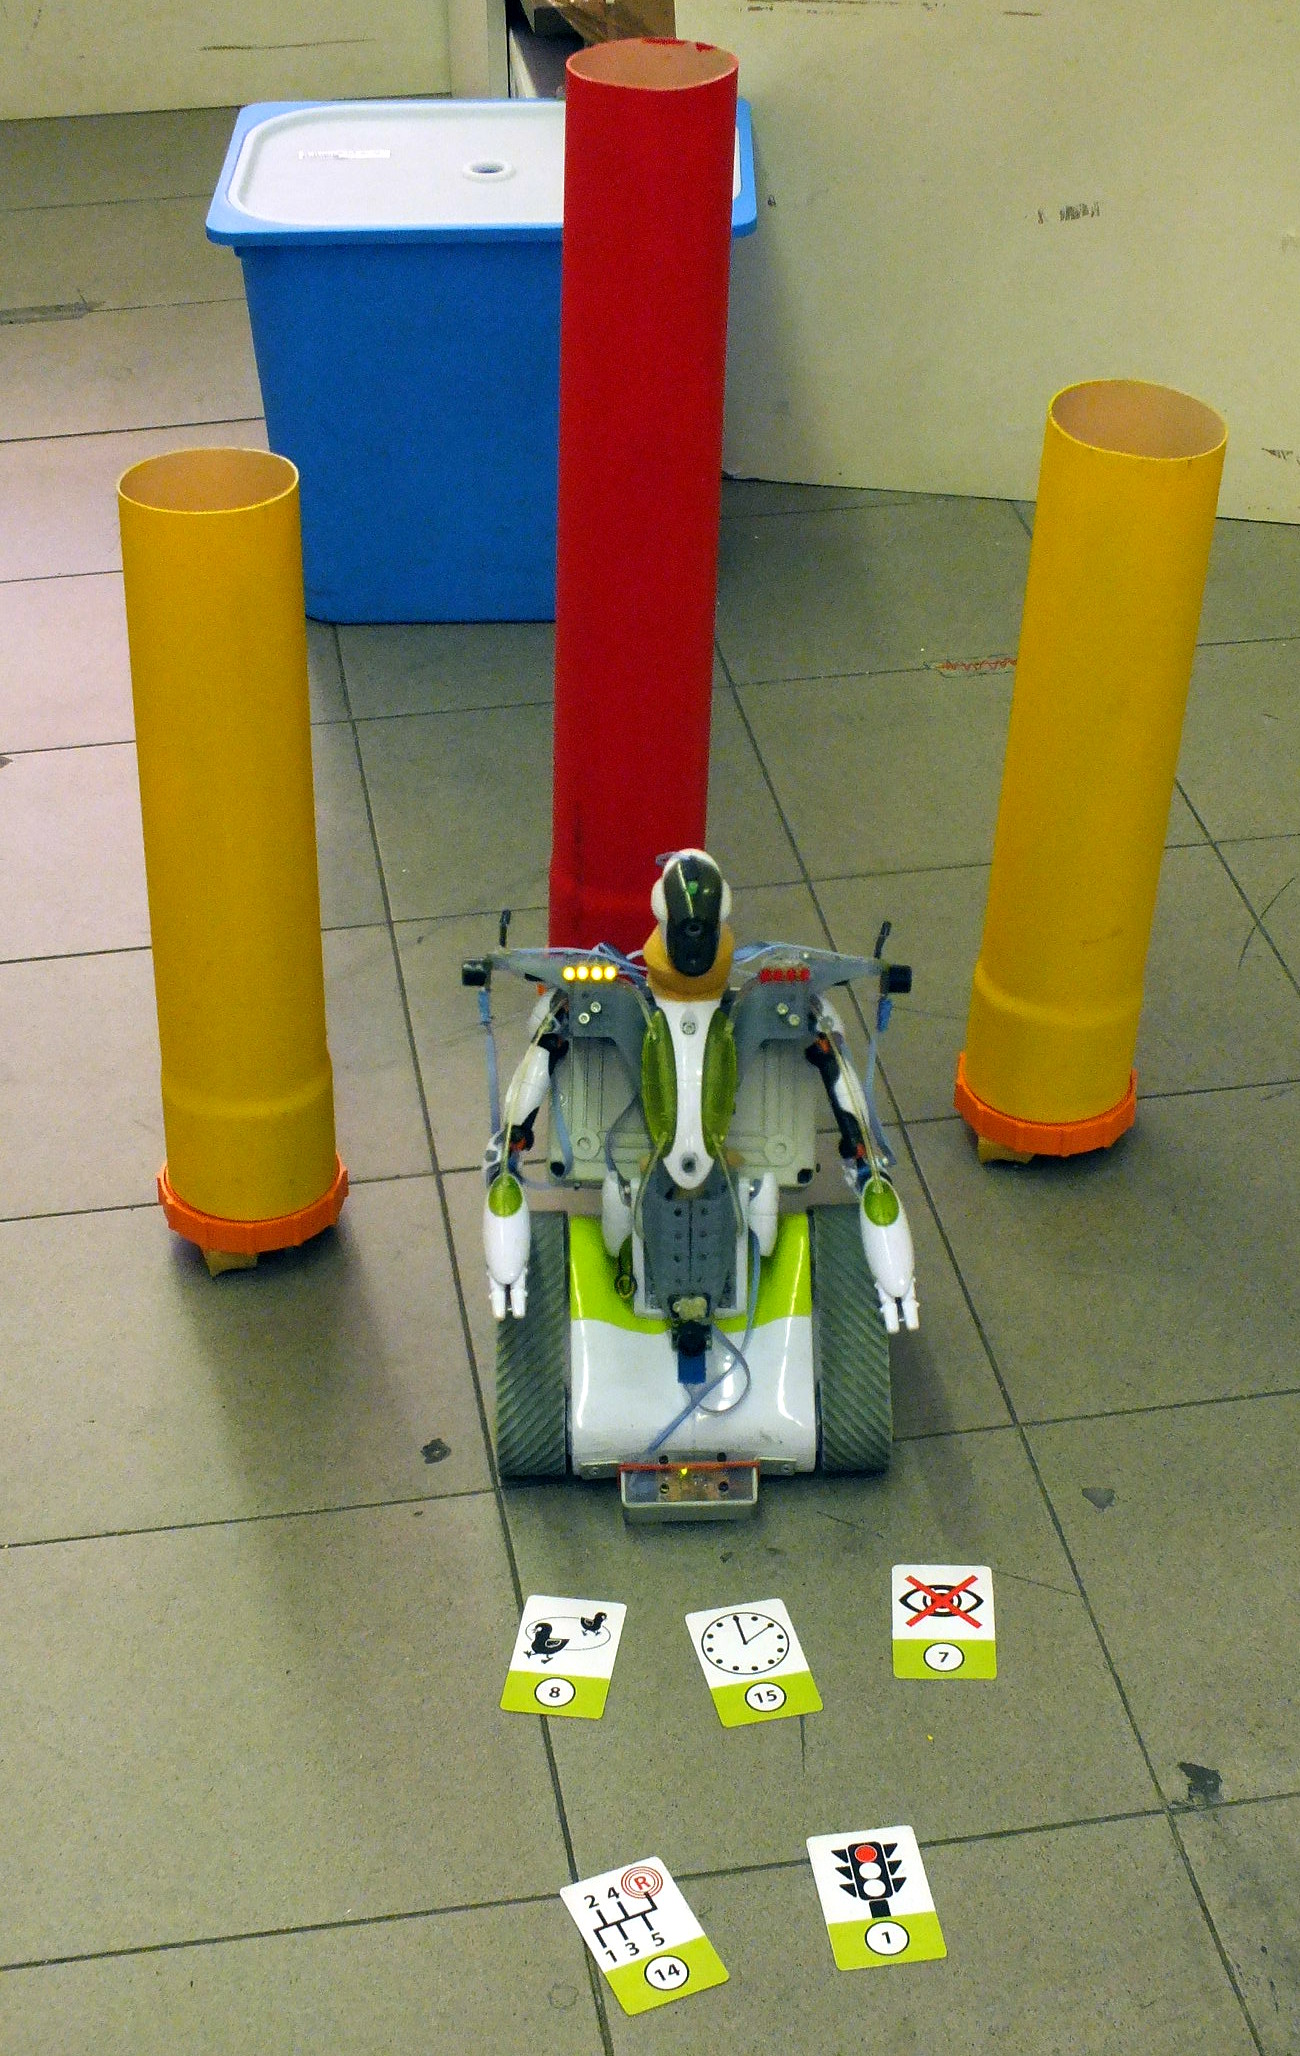
\includegraphics[scale=0.13]{images/spykeecontorri}
\caption{Spykee, con due fabbriche, una torre e alcune delle carte trappola}
\end{figure}

Poiché nel gioco viene già utilizzata una telecamera per poter riconoscere alcuni oggetti, inizialmente si è pensato di implementare anche le trappole utilizzando meccanismi di visione artificiale. In particolare, sono stati presi in considerazione vari tipi di marker bidimensionali, in particolare i ``Data Matrix'' e i tag della libreria ``ARToolkitPlus''\footnote{A differenza dei codici Data Matrix, che sono pensati per contenere informazioni arbitrarie, ad esempio URL oppure informazioni di spedizione, i tag ARToolkitPlus codificano solo un id, e sono pensati per applicazioni di identificazione, localizzazione, \dots (anche in presenza di distorsioni nell'immagine o altre condizioni non ottimali).}. Purtroppo, tutti questi meccanismi hanno dato scarsi risultati in termini di velocità oppure di qualità del riconoscimento. I difetti riscontrati sono, ad esempio, un'enorme dipendenza dalle condizioni di luce, scarsi risultati in movimento, dovuti anche alla lentezza degli algoritmi (specialmente nel caso dei Data Matrix), e alle pessime condizioni delle immagini catturate. Per questi motivi, le soluzioni basate sul riconoscimento di tag mediante visione sono state scartate.

Una soluzione che ha fornito prestazioni migliori, e che è stata adottata per l'implementazione del gioco, è l'uso di tag RFID passivi a 125 KHz, che tuttavia richiede l'aggiunta di ulteriore hardware. I tag vengono correttamente riconosciuti quando il robot passa sopra di essi, con un margine di errore accettabile. Inoltre, il loro formato (tessere di plastica della dimensione di una carta di credito, che eventualmente l'utente può facilmente identificare con delle etichette) li rende abbastanza comodi per l'utilizzo da parte del giocatore. Per la lettura dei tag, è stato montato sul robot il lettore ID-12 della ID-Innovations. Il lettore trasmette alla scheda di controllo presente sul robot i dati (id del tag letto più un checksum) in formato testuale tramite un collegamento seriale a 9600 bps. Una limitazione di questo specifico modello di lettore è la presenza di un'antenna interna, che ne limita pesantemente il posizionamento.

\section{Torri e fabbriche}

Le torri e le fabbriche sono costituite semplicemente da tubi di PVC leggero di diametro $100$ mm. Le fabbriche, di altezza $45$ cm, sono state verniciate di giallo, mentre le torri, alte $60$ cm, sono di colore rosso.

La base dei cilindri è costituita da un tappo su cui è montato un interruttore che risulta chiuso quando il tubo è appoggiato a terra, e viene aperto quando il cilindro viene abbattuto. L'apertura dell'interruttore attiva un trasmettitore (del tipo di quelli utilizzati per comandare i cancelli elettrici) che invia un segnale radio a un ricevitore posto sul robot. Quest'ultimo segnala l'evento all'unità di elaborazione.

Il ricevitore montato sul robot è il RX-4M-HCS prodotto dall'Aurel, ed è dotato di quattro canali separati con uscita open-drain (corrispondenti ai quattro pulsanti presenti sui corrispondenti trasmettitori, sempre della stessa marca). Pertanto, si sono impostati i relativi ingressi del microcontrollore come ingressi pull-up. Le uscite del ricevitore sono state impostate in modalità monostabile: in questo modo, ogni volta che una torre o una fabbrica cade, viene inviato un segnale al microcontrollore presente sul robot, e quindi all'unità di elaborazione.